
In order to explain some failures of the standard model, the 2HDM 
postulated existence of an additional Higgs doublet. It leads to two 
charged and three neutral physical scalar particles. A charged Higgs 
boson decays to various channels depending on the parameter space 
corresponding to its mass and $\tan\beta$. A search for the charged 
Higgs in the $H^+ \to c\bar{s}$ channel has been performed in this 
analysis with the data collected by the CMS experiment at the 
center-of-mass energy of 13 \TeV with an integrated luminosity of 
35.9\fbinv. The observed data and standard model predictions are in 
agreement within the statistical and systematic uncertainties. That is, 
no signal has been observed in the data for the mass of charged Higgs 
in the range 80 to 160 \GeV. In the absence of an excess, a 95\% CL 
upper limit has been put on \brThb, assuming \brHcs = 100\%. The 
kinematic fitting and a new technique which uses \PQc tagging has been 
intensively exploited to improve the limits. The final limits from 
combined charm categories are shown in Tables 
\ref{tab:limit_muon_ele} and \ref{tab:limit_lepton}. The observed 
limits are in the range 0.32--2.44\%, 0.26--2.77\%, and 0.26--1.68\% 
for \mujets, \ejets, and \ljets channel, respectively. The observed 
limits at 13 \TeV are better by an average factor of 7.6 as compared 
to the earlier CMS results at 8 \TeV~\cite{Khachatryan:2015uua}. The 
improvement in the limit is partly due to higher luminosity and partly 
due the new technique used in this analysis. 

\begin{figure}
    \centering
    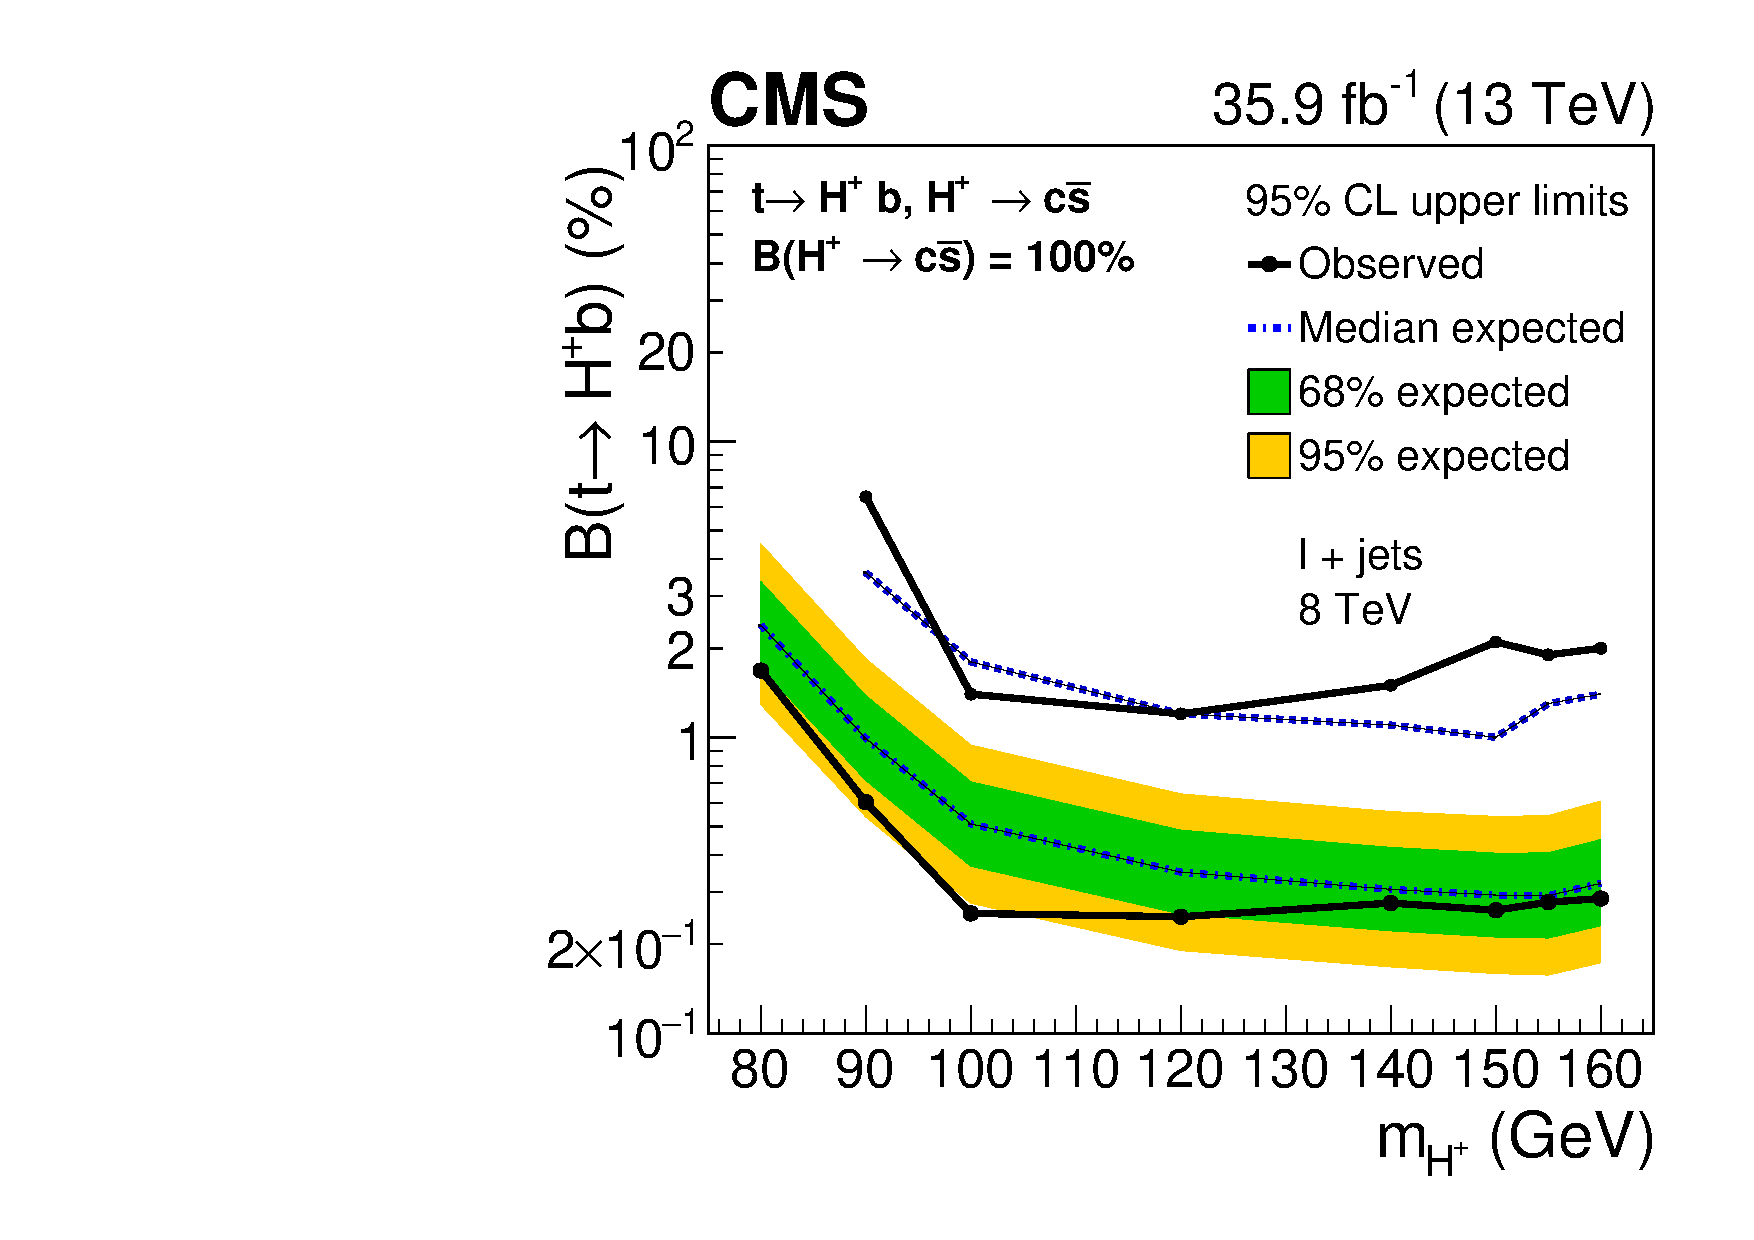
\includegraphics[width=0.5\linewidth]{Image/Limit/limit_8TeV_vs_13TeV.pdf}
    \caption{The upper limit on \brThb as a function of \mHp for \ljets 
        channel. The limits from 13 \TeV analysis (lower curves) are 
        obtained by combining exclusive charm categories. The limits 
        from 8 \TeV analysis (upper curves) were obtained from inclusive 
        events without applying charm tagging. The 80 \GeV signal mass 
        point was not considered at 8 \TeV analysis.}
\label{fig:limit_8TeV_vs_13TeV}
\end{figure}

\renewcommand{\arraystretch}{1.2}
\begin{table*}[ht]
\centering
\topcaption{Expected and observed 95\% \CL exclusion limits in \% on
    \Bthb in the muon\,+\,jets
    (electron\,+\,jets) channel, after the individual charm tagging categories have
    been combined.}
\label{tab:limit_muon_ele}
\begin{scotch}{ccccccc}
\multirow{2}{*}{$\mhp$ (\GeVns)} & \multicolumn{5}{c}{Expected} & \multirow{2}{*}{Observed} \\
& $-2\sigma$ & $-1\sigma$ & median & $+1\sigma$ & $+2\sigma$ &\\
\hline
80  & 1.58 (1.96) & 2.10 (2.61) & 2.95 (3.63) & 4.16 (5.10) & 5.61 (6.84) & 2.44 (2.77)\\
90  & 0.69 (0.79) & 0.92 (1.06) & 1.28 (1.47) & 1.79 (2.05) & 2.39 (2.74) & 0.72 (1.38)\\
100 & 0.35 (0.42) & 0.46 (0.56) & 0.64 (0.77) & 0.90 (1.08) & 1.19 (1.43) & 0.34 (0.53)\\
120 & 0.24 (0.28) & 0.32 (0.37) & 0.44 (0.52) & 0.61 (0.72) & 0.82 (0.95) & 0.32 (0.44)\\
140 & 0.21 (0.24) & 0.28 (0.32) & 0.39 (0.44) & 0.54 (0.61) & 0.72 (0.81) & 0.47 (0.32)\\
150 & 0.20 (0.23) & 0.27 (0.31) & 0.37 (0.43) & 0.52 (0.60) & 0.69 (0.80) & 0.52 (0.26)\\
155 & 0.20 (0.23) & 0.27 (0.31) & 0.38 (0.42) & 0.53 (0.60) & 0.71 (0.80) & 0.57 (0.26)\\
160 & 0.22 (0.26) & 0.30 (0.35) & 0.42 (0.48) & 0.59 (0.68) & 0.80 (0.92) & 0.53 (0.32)\\
\end{scotch}
\end{table*}

\begin{table}[ht]
\centering
\topcaption{Expected and observed 95\% \CL exclusion limits in \% on
    \Bthb, after the individual charm
    tagging categories and the muon and electron channels have been
    combined.}
\label{tab:limit_lepton}
\begin{scotch}{ccccccc}
\multirow{2}{*}{$\mhp$ (\GeVns)} & \multicolumn{5}{c}{Expected} & \multirow{2}{*}{Observed} \\
& $-2\sigma$ & $-1\sigma$ & median & $+1\sigma$ & $+2\sigma$ & \\
\hline
80  & 1.29 & 1.72 & 2.39 & 3.36 & 4.50 & 1.68\\
90  & 0.54 & 0.72 & 0.99 & 1.38 & 1.84 & 0.60\\
100 & 0.28 & 0.37 & 0.51 & 0.71 & 0.94 & 0.25\\
120 & 0.19 & 0.25 & 0.35 & 0.49 & 0.64 & 0.25\\
140 & 0.17 & 0.22 & 0.31 & 0.42 & 0.56 & 0.28\\
150 & 0.16 & 0.21 & 0.29 & 0.41 & 0.54 & 0.26\\
155 & 0.16 & 0.21 & 0.29 & 0.41 & 0.54 & 0.28\\
160 & 0.17 & 0.23 & 0.32 & 0.45 & 0.61 & 0.29\\
\end{scotch}
\end{table}
